\documentclass{standalone}
\usepackage{tikz}
\usepackage{pgf}
% \usepackage{luatex85}
\usetikzlibrary{graphs, shapes}
% \usetikzlibrary{graphdrawing}
% \usegdlibrary{layered}


\pgfdeclareradialshading{ballshading}{\pgfpoint{-12bp}{10bp}}
{color(0bp)=(yellow!15!white);
color(5bp)=(yellow!15!white);
color(6bp)=(yellow);
% color(18bp)=(yellow!70!black);
% color(25bp)=(yellow!50!black);
color(50bp)=(black!70!green)
}

\pgfdeclareradialshading{ballshading1}{\pgfpoint{-12bp}{10bp}}
{color(0bp)=(orange!15!white);
color(5bp)=(orange!15!white);
color(6bp)=(orange);
% color(18bp)=(orange!70!black);
% color(25bp)=(orange!50!black);
color(50bp)=(black!70!orange)
}

\pgfdeclareradialshading{ballshading2}{\pgfpoint{-12bp}{10bp}}
{color(0bp)=(red!15!white);
color(5bp)=(red!15!white);
color(6bp)=(red);
% color(18bp)=(red!70!black);
% color(25bp)=(red!50!black);
color(50bp)=(black!70!red)
}

% \tikzstyle{type0} = [circle, shading=ball, ball color=yellow, draw=yellow!50!red, thick, label=0]
\tikzstyle{0} = [shading=ballshading, draw=green!70!red, thick, label={center:0}, minimum size=5mm]
\tikzstyle{1} = [shading=ballshading1, draw=yellow!50!red, thick, label={center:1}, minimum size=5mm]
\tikzstyle{2} = [shading=ballshading2, draw=black!90!red, thick, label={center:2}, minimum size=5mm]
% \tikzstyle{2} = [shading=ballshading2,circle, draw=black!90!red, thick, label={center:2}, minimum size=5mm]
% \tikzstyle{2} = [circle, fill=white!90!red, draw=yellow!50!red, thick, label=2]
\begin{document}
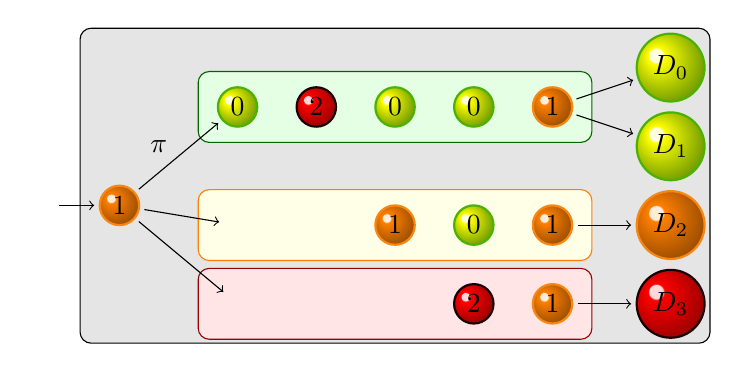
\begin{tikzpicture}[
  % -!-,
  every node/.style={circle, outer sep=2pt},
  % layered layout,
  centered,
  new set=type0,
  new set=type1,
  new set=type2
  ]
  % \node (0-1) at (10,0) {hey};
   % \foreach \x [count = \i] in {2,...,5}
     % \node (0-\x) [left of=0-\i] {\x};
  % \graph [trie, grow right]
  % { "$\pi$" ->[red,"foo"] {
  %   "" -!- "" [1] -!- "" [0] -!- "" [0] -!- ""[2] ->
  %   {
  %     "$D_0$" [0],
  %     "$D_1$" [0]
  %   },
  %   "" -!- "" -!- "" [1] -!- ""[1] -!- ""[0] ->
  %   {
  %     "$D_2$" [1]
  %   },
  %   "" -!- "" -!- "" -!- ""[2] -!- ""[1] ->
  %   {
  %     "$D_3$" [2]
  %   },
  %   }
  % };
  \draw [rounded corners, fill=black!10!white, draw=black] (-2.5, 0.5) rectangle (5.5,4.5);

  \node [set=type0, shading=ballshading, draw=green!70!red, thick] at (5,4) {$D_0$};
  \node [set=type0, shading=ballshading, draw=green!70!red, thick] at (5,3) {$D_1$};
  \node [set=type1, shading=ballshading1, draw=yellow!50!red, thick] at (5,2) {$D_2$};
  \node [set=type2, shading=ballshading2, draw=black!90!red, thick] at (5,1) {$D_3$};

  \draw [rounded corners, fill=green!10!white, draw=green!40!black] (-1, 3.05) rectangle (4,3.95);

  \node (q00) [1] at (3.5, 3.5) {};
  \node (q01) [0, left of=q00] {};
  \node (q02) [0, left of=q01] {};
  \node (q03) [2, left of=q02] {};
  \node (q04) [0, left of=q03] {};

  \draw [rounded corners, fill=yellow!10!white, draw=orange] (-1, 1.55) rectangle (4,2.45);

  \node (q10) [1] at (3.5, 2) {};
  \node (q11) [0, left of=q10] {};
  \node (q12) [1, left of=q11] {};
  \node (q13) [left of=q12] {};
  \node (q14) [left of=q13] {};

  \draw [rounded corners, fill=red!10!white, draw=red!60!black] (-1, 0.55) rectangle (4, 1.45);

  \node (q20) [1] at (3.5, 1) {};
  \node (q21) [2, left of=q20] {};
  \node (q22) [left of=q21] {};
  \node (q23) [left of=q22] {};
  \node (q24) [left of=q23] {};

  \node (new) [1] at (-2, 2.25) {};
  \node (out) at (-3, 2.25) {};
  \node () [inner sep=0pt, outer sep=0pt, radius=0pt] at (-1.5, 3) {$\pi$};

  \graph {
    (q00) -> (type0);
    (q10) -> (type1);
    (q20) -> (type2);
    (out) -> (new) -> {
      (q04);
      (q14);
      (q24)
    };
  };
  %\node (d0) [fill=red] at (11,0) {$D_0$};
  %\node [fill=white!80!red, x radius=1pt, y radius=2pt, shift={(-3pt,1pt)}] at (11,0) {};
  % \node (d1) [type1, above of=d0] {$D_1$};
  %\node (d2) [above of=d1] {$D_2$};
  %\node (d3) [above of=d2] {$D_3$};
  % \filldraw (11,0) circle [line width=1pt,radius=1, fill=red];
  % \filldraw (11,0) circle [fill=white!80!red, x radius=0.2, y radius=0.3,rotate=-35, shift={(-0.6,0)}];
  % \filldraw (4,0) circle (.5cm) (4.5,0) circle (.5cm);
  % \path (10,0) edge [draw, dashed] (10, 2);



  

\end{tikzpicture}

\end{document}
